\documentclass[twocolumn,a4paper,dvipdfmx]{ieicejsp}
\usepackage[T1]{fontenc}
\usepackage{lmodern}
\usepackage{textcomp}
\usepackage{latexsym}
\usepackage{float}
\usepackage{graphicx}
\usepackage{amsmath, amssymb}
\usepackage{bm}
\usepackage{upgreek}
\usepackage{caption}
\usepackage{booktabs}
\usepackage{multirow}
\usepackage{url}
\usepackage{algorithm}
\usepackage{algpseudocode}
\usepackage{xcolor}

\captionsetup{font=small}
\renewcommand{\dbltopfraction}{0.9}
\renewcommand{\topfraction}{0.9}
\renewcommand{\textfraction}{0.1}
\setcounter{dbltopnumber}{2}
\DeclareMathOperator*{\argmax}{arg\,max}
% 修正箇所を赤字で示すコマンド
\newcommand{\add}[1]{{\color{red}#1}}

\title{
    {{\bf WordNetの上位語への確率の集約による\\再学習なしの粒度可変アノテーション}
    {\normalsize \\ Retraining-Free Adjustable-Granularity Annotation by Aggregating Probabilities over WordNet Hypernyms}}
}
\author{
    著者名 \\ Author Name
}
\affliate{%
    所属機関名 \\
    Affiliation \\
}

\begin{document}
\maketitle

\begin{abstract}
本稿では，モデルの再学習を行わずに，学習時に無い物体を検出し，粗い語から細かい語までの確信度に応じた粒度で命名する粒度可変アノテーションを提案する．
提案手法は，COCOで学習したYOLO11xのボックスにOWLv2の物体らしさの上位の領域を加え，領域の特徴から求めた7806語の確率をWordNetの上位語へ集約し，集約した確率が閾値以上の間だけ上位語から下位語へ進む．
さらに，各アノテーションと経路上の各単語に，検証用の画像のみで14個の重みを求めた正しさの確率をスコアとして付け，利用者がスコアの閾値によって出力の数と粒度を選べるようにする．
LVISの人手の注釈を学習に用いていないOWLv2を用い，LVISのアノテーションでCOCO外の物体を評価した結果，COCO外の物体の検出は56.0\%，正しい上位語・下位語による命名は21.1\%であった．
COCO外の物体と対応した同じ領域に対し，正しく命名できた割合は，確率が最大の1語を出力する場合の25.9\%に対し提案手法で43.0\%であった．
提案したスコアは，検出のスコアのみを用いる場合と比べ，全ての誤りを数えるAPを0.171から0.197に高め，期待校正誤差を0.145から0.028に下げた．
一方，LVISのカテゴリまで正しい出力のみを数えるAPでは1語を出力する方法が上回り，評価の語彙を事前に与えた場合には集約の効果は無かった．
また，加えた領域の出力の多くは物体の一部や背景に対するものであり，精度を制限する主な要因は命名よりも領域の追加にあることを示した．
予備実験として，COCOの80クラスの範囲では，切り抜き画像に対するCLIPとSigLIPのラベルの一致率は0.56〜0.58であり，COCOで学習した物体認識モデル自身の0.96〜0.97に大きく劣ることも示した．
\end{abstract}

\noindent
{\bf キーワード：}粒度可変アノテーション，WordNet，文章・画像埋め込みモデル，CLIP，SigLIP，YOLO，DETR，OWLv2，オープンボキャブラリ，校正

\section{はじめに}
画像中の物体に対するアノテーションは，物体の位置を表すバウンディングボックスと，物体が何であるかを表すクラスの組から構成される．
YOLO\cite{ref_YOLO}やDetection Transformer（DETR）\cite{ref_DETR}に代表される物体認識モデルは，あらかじめ定めたクラスの集合で学習されるため，学習時のクラスの範囲では高い精度で物体を認識できる．
一方，学習時に定めたクラスより細かい粒度，例えば「dog」に対する犬種のようなクラスを付けるためには，そのクラスを含むデータでモデルを学習し直す必要がある．

画像と文章を同じ空間に埋め込むContrastive Language-Image Pre-training（CLIP）\cite{ref_CLIP}やSigLIP\cite{ref_SigLIP}のような文章・画像埋め込みモデルを用いると，任意の単語と画像の類似度を追加の学習なしに計算できる．
また，語彙の上位語と下位語の関係を記述したWordNet\cite{ref_WordNet}を用いると，ある単語より細かい粒度の単語の集合を得ることができる．
OWL-ViT\cite{ref_OWLViT}やOWLv2\cite{ref_OWLv2}のようなオープンボキャブラリの物体認識モデルは，これらの埋め込みを用いて，テキストで与えたクラスの物体を検出できる．
しかし，通常はアノテーションに用いるクラスの集合を利用者が事前に与える必要があり，学習時に無い物体を数千語の語彙から1語で命名すると，誤りが多い．
例えば4.4節で示すように，LVIS\cite{ref_LVIS}の人手の注釈を学習に用いていないOWLv2では，COCO外の物体に対する7806語からの1位の単語の正解率は18.0\%であった．
一方，正しい単語が1位でなくても，その上位語（例えばparkaに対するjacketやclothing）は正しいことが多い．
したがって，学習時に無い物体に対しては，常に細かい1語を出力するのではなく，正しい可能性が高い最も細かい語を選び，その正しさの確率を付けることが望ましい．

本稿では，物体認識モデルとオープンボキャブラリの物体認識モデルの領域の特徴，およびWordNetを組み合わせ，モデルの再学習を行わずに，学習時に無い物体を検出し，粗い語から細かい語までの粒度で命名する粒度可変アノテーションを提案する．
提案手法は，領域の特徴から求めた語彙全体の確率をWordNetの上位語へ集約し，集約した確率が閾値以上の間だけ上位語から下位語へ進むことで，確信度に応じた粒度の単語を選ぶ．
さらに，各アノテーションと，粗い語から選んだ単語までの経路上の各単語に，正しさの確率を表すスコアを付ける．
これにより，利用者はスコアの閾値によって，出力の数と粒度を必要な正解率に応じて選ぶことができる．
スコアの重みは検証用の画像のみで求める14個であり，物体認識モデルと埋め込みモデルは再学習しない．

本稿の貢献は以下の3点である．
第一に，再学習なしで学習時に無い物体を検出し，確信度に応じた粒度で命名する手法と，そのアノテーションおよび経路上の各単語の正しさの確率を求める方法を定式化する．
第二に，WordNetのSynsetが付与されたLVISのアノテーションと，評価に用いるカテゴリを学習時に見ていない重みを用いて，COCO外の物体に対する性能を評価する．
その際，階層を用いずに1語を選ぶ方法や，評価の語彙を事前に与える方法と比較し，階層的な指標とラベルの正誤のみによる指標の両方を，ブートストラップによる信頼区間とともに示す．
第三に，誤りを種類ごとに分解し，提案手法の精度を制限する要因が，物体でない領域や物体の一部への命名にあることを示す．
また，予備実験として，COCOの80クラスの範囲で切り抜き画像と文章・画像埋め込みモデルによるクラスの推定を評価し，学習時のクラスの範囲では物体認識モデル自身のクラスを用いるべきであることを示す．

本稿の構成は以下のとおりである．
2章で関連研究，3章で提案手法を述べる．
4章では，予備実験と，COCO外の物体に対する評価の結果を示す．
5章で考察を行い，6章で本稿をまとめる．

\section{関連研究}
\subsection{物体認識モデル}
YOLO\cite{ref_YOLO}は画像を格子に分割し，各格子からボックスとクラスを1回の推論で予測する．
本稿ではYOLOの系列のYOLO11x\cite{ref_YOLO11}を用いる．
DETR\cite{ref_DETR}はTransformerによる集合予測として物体認識を定式化し，重複するボックスの除去を行わずにボックスとクラスを出力する．
いずれもCOCO\cite{ref_COCO}の80クラスで学習されたモデルが公開されており，学習時のクラス以外を出力することはできない．

\subsection{文章・画像埋め込みモデル}
CLIP\cite{ref_CLIP}は画像と文章の対の対照学習により，画像エンコーダとテキストエンコーダを同じ空間に埋め込む．
SigLIP\cite{ref_SigLIP}は，対照学習の目的関数を，候補全体で正規化するソフトマックスから，画像と文章の対ごとのシグモイドに置き換えたモデルである．
いずれも，クラス名を「a photo of a 〇〇」のような文章に埋め込み，画像との類似度を比較することで，追加の学習なしに任意のクラスへの分類（ゼロショット分類）を行うことができる．
OWL-ViT\cite{ref_OWLViT}やGrounding DINO\cite{ref_GroundingDINO}は，このような埋め込みを物体認識に組み込み，テキストで指定したクラスの物体を検出する．
本稿は，物体認識モデルと文章・画像埋め込みモデルを組み合わせ，ボックスの検出は物体認識モデルで1回だけ行い，クラスの推定を文章・画像埋め込みモデルで繰り返す点で，これらのモデルと異なる．

\subsection{WordNet}
WordNet\cite{ref_WordNet}は英語の名詞を同義語の集合（Synset）にまとめ，Synsetの間の上位語・下位語の関係を記述した語彙データベースである．
例えばdogのSynsetの下位語にはworking dogやhunting dog等が含まれ，下位語を順にたどることで細かい粒度の単語が得られる．
名詞のSynsetは，最上位のカテゴリ（unique beginner）を根とする木構造をなしている．

\subsection{階層的な分類と確信度}
確信度が低い場合に粗いクラスを出力する考え方は，画像分類において正解率と細かさのトレードオフとして定式化されている\cite{ref_Hedging}．
Dengらは，クラスの階層上で正解率の下限を満たしつつ情報量が最大となるクラスを選ぶ方法を提案した．
また，CHiLS\cite{ref_CHiLS}は，ゼロショット分類において，各クラスの下位のクラスの名前を文章・画像埋め込みモデルに与え，その確率を上位のクラスへ集約することで正解率を改善した．
これらはいずれも画像全体のクラスが事前に定めた集合に含まれる分類の問題であり，本稿は，検出を伴い，学習時に無い物体に7806語のWordNetの語彙から粒度を選んで命名する点で異なる．
出力の確率を正解率と一致させる校正には，ロジスティック回帰による方法\cite{ref_Platt}や温度によるスケーリング\cite{ref_Calibration}があり，校正の程度は期待校正誤差で評価される\cite{ref_Calibration}．

\section{提案手法}
\subsection{基本の手法：切り抜き画像による粒度可変アノテーション}
本節では，学習時のクラスの範囲を対象とする基本の手法を述べ，4.2節の予備実験に用いる．
学習時に無い物体を対象とする提案手法は3.3節で述べる．
画像$ {\mathbf X} \in {\mathbb R}^{H \times W \times 3} $に対し，物体認識モデル$ D $はボックスの集合$ {\mathbb B} = \{ {\mathbf b}_1, {\mathbf b}_2, \ldots \} = D({\mathbf X}) $を出力する．
ここで，$ H $，$ W $は画像の高さと幅，$ {\mathbf b}_i \in {\mathbb R}^4 $は$ i $番目の物体のボックスの左上と右下の座標である．
$ i $番目の物体の切り抜き画像を

\begin{equation}
    {\mathbf X}_i = \mathrm{Pad} \bigl( \mathrm{Crop}({\mathbf X}, {\mathbf b}_i) \bigr)
    \label{eq_crop}
\end{equation}

\noindent
とする．
ここで，$ \mathrm{Crop}({\mathbf X}, {\mathbf b}) $は画像$ {\mathbf X} $から$ {\mathbf b} $の範囲を切り抜く関数，$ \mathrm{Pad}(\cdot) $は長辺に合わせて黒で埋めて正方形にする関数であり，文章・画像埋め込みモデルの前処理で物体の両端が失われないようにするために用いる．

文章・画像埋め込みモデル$ F $は，画像と文章をそれぞれ$ D' $次元のL2正規化された特徴ベクトルに埋め込む．
切り抜き画像の特徴ベクトルを$ {\mathbf v}_{{\mathbf X}_i} = F({\mathbf X}_i) $，単語$ w $の特徴ベクトルを，単語を「a photo of a $ \{w\} $」という文章に埋め込んだ$ {\mathbf v}_w = F(t(w)) $とし，両者の類似度をコサイン類似度

\begin{equation}
    \mathrm{sim}({\mathbf v}_{{\mathbf X}_i}, {\mathbf v}_w) = {\mathbf v}_{{\mathbf X}_i} {\mathbf v}_w^{\top}
    \label{eq_similarity}
\end{equation}

\noindent
とする．
ここで，$ t(w) $は単語$ w $を文章に埋め込む関数である．

語彙レベルが最も高い単語の集合を$ {\mathbb W} = \{ w_1, w_2, \ldots \} $とする．
提案手法は，切り抜き画像と最も類似した単語

\begin{equation}
    j^\ast = \argmax_{j} \mathrm{sim}({\mathbf v}_{{\mathbf X}_i}, {\mathbf v}_{w_j})
    \label{eq_argmax}
\end{equation}

\noindent
を選び，類似度が類似と判断する下限値$ \theta $以上であれば，ボックスと単語の組$ ({\mathbf b}_i, w_{j^\ast}) $を出力する．
その後，単語の集合$ {\mathbb W} $を$ w_{j^\ast} $の下位語からなる集合に置き換え，(\ref{eq_argmax})による選択を繰り返す．
類似度が$ \theta $未満となるか，下位語が存在しなくなった時点で，$ i $番目のボックスのアノテーションを終了する．
これにより，1つのボックスに対し，粗い語から細かい語までの単語の列が出力される．
全体の手順をAlgorithm \ref{alg_granular}に示す．

\begin{algorithm}[t]
    \caption{粒度可変アノテーション}
    \label{alg_granular}
    \begin{algorithmic}[1]
        \Require 物体認識モデル$ D $，文章・画像埋め込みモデル$ F $，語彙レベルが最も高い単語の集合$ {\mathbb W} $，画像$ {\mathbf X} $，類似と判断する下限値$ \theta $
        \State $ {\mathbb B} = \{ {\mathbf b}_1, {\mathbf b}_2, \ldots \} \gets D({\mathbf X}) $
        \For{$ i = 1, 2, \ldots $}
            \State $ {\mathbf X}_i \gets \mathrm{Pad}(\mathrm{Crop}({\mathbf X}, {\mathbf b}_i)) $，$ {\mathbf v}_{{\mathbf X}_i} \gets F({\mathbf X}_i) $
            \State $ {\mathbb W}_i \gets {\mathbb W} $
            \Loop
                \State $ j^\ast \gets \argmax_j \mathrm{sim}({\mathbf v}_{{\mathbf X}_i}, F(t(w_j))) $，$ w_j \in {\mathbb W}_i $
                \If{$ \mathrm{sim}({\mathbf v}_{{\mathbf X}_i}, F(t(w_{j^\ast}))) < \theta $}
                    \State \textbf{break}
                \EndIf
                \State 出力 $ ({\mathbf b}_i, w_{j^\ast}) $
                \State $ {\mathbb W}_i \gets w_{j^\ast} $の下位語からなる集合
                \If{$ {\mathbb W}_i = \emptyset $}
                    \State \textbf{break}
                \EndIf
            \EndLoop
        \EndFor
    \end{algorithmic}
\end{algorithm}

\subsection{基本の手法の実装}
物体認識モデル$ D $には，COCOの80クラスで学習済みのYOLO11x\cite{ref_YOLO11}と，DETR（ResNet-50）\cite{ref_DETR}を用いる．
YOLO11xは検出スコアが0.25以上，DETRは「物体なし」以外のクラスの最大確率が0.5以上のボックスを用いる．
文章・画像埋め込みモデル$ F $には，OpenCLIP\cite{ref_OpenCLIP}によるCLIP ViT-B/32（OpenAIの学習済みの重み）と，SigLIP ViT-B/16（WebLIで学習済みの重み）を用いる．
下位語の集合は，WordNetにおける選んだ単語のSynsetの直接の下位語とし，各Synsetの先頭のレンマを単語とする．

\subsection{提案手法：学習時に無い物体への粒度可変アノテーション}
Algorithm \ref{alg_granular}をそのまま用いると，COCOで学習した物体認識モデル$ D $はCOCO外の物体を背景として扱うことがあり，検出されなかった物体には単語を付けられない．
また，4.2節で示すように，WordNetの上位語から下位語を1段ずつたどると，最初の段階や役割を表す下位語で誤りやすい．
そこで，モデルの再学習を行わずに，学習時に無い物体を検出し，学習時に無い語彙で命名するため，Algorithm \ref{alg_granular}を以下のように拡張する．

{\bf A1：物体認識モデルのクラスの利用．}
$ D $が出力したボックス$ {\mathbf b}_i $には，$ D $のクラス$ y_i $を出力する．

{\bf A2：領域の追加と棄却．}
テキストに依存しない物体らしさのスコア$ o({\mathbf b}) $を出力するOWLv2\cite{ref_OWLv2}の領域$ {\mathbb B}_{\mathrm{O}} $のうち，$ D $のボックス$ {\mathbb B} $のいずれともIoUが0.5未満の領域を，スコアが下限値$ o_{\min} $以上のものに限りスコアの上位$ K $件まで加える．

\begin{equation}
    \begin{aligned}
    {\mathbb B}' = {\mathbb B} \cup \mathrm{Top}_K \Bigl\{ {\mathbf b} \in {\mathbb B}_{\mathrm{O}} \Bigm| & \max_{{\mathbf b}' \in {\mathbb B}} \mathrm{IoU}({\mathbf b}, {\mathbf b}') < 0.5, \\
    & o({\mathbf b}) \geq o_{\min} \Bigr\}
    \end{aligned}
    \label{eq_add}
\end{equation}

{\bf N1：領域の特徴による語彙全体の確率．}
加えた領域$ {\mathbf b} $の単語は，切り抜き画像ではなく，OWLv2が領域ごとに出力する特徴から求める．
語彙$ {\mathbb V} $は，物理的な実体（physical entity）の下位のSynsetのうち，COCO train2017のキャプションに5回以上出現するレンマを持つもの（7806語）とする．
OWLv2が領域$ {\mathbf b} $に対して出力するL2正規化された埋め込みを$ {\mathbf e}_{\mathbf b} $，ロジットの倍率を$ s_{\mathbf b} $，単語$ w $の文章の特徴を$ {\mathbf u}_w $とし，語彙全体で正規化した確率を

\begin{equation}
    p(w \mid {\mathbf b}) = \frac{\exp \bigl( \beta s_{\mathbf b} {\mathbf e}_{\mathbf b} {\mathbf u}_w^{\top} \bigr)}{\sum_{w' \in {\mathbb V}} \exp \bigl( \beta s_{\mathbf b} {\mathbf e}_{\mathbf b} {\mathbf u}_{w'}^{\top} \bigr)}
    \label{eq_prob}
\end{equation}

\noindent
とする．
ここで，$ \beta $は確率の鋭さを調整する温度の倍率である．
OWLv2の倍率$ s_{\mathbf b} $のままでは7806語の確率がほぼ一様になるため，$ \beta $を検証用の画像で選ぶ．

{\bf N2：上位語への確率の集約．}
各単語の確率をWordNetの上位語へ足し上げ，Synset $ n $の確率を

\begin{equation}
    q(n \mid {\mathbf b}) = \sum_{w \in {\mathbb V}} p(w \mid {\mathbf b}) \, {\mathbf 1}\bigl[ n \in \mathrm{Anc}(w) \bigr]
    \label{eq_aggregate}
\end{equation}

\noindent
とする．
ここで，$ \mathrm{Anc}(w) $は$ w $自身とその全ての上位語の集合，$ {\mathbf 1}[\cdot] $は条件を満たす場合に1，それ以外で0となる関数である．
$ q $は上位語ほど大きく，根のSynsetで1となる．

{\bf N3：上位語からの貪欲な選択．}
根のSynset $ n_0 $（physical entity）から出発し，集約した確率が最大の直接の下位語

\begin{equation}
    n_{k+1} = \argmax_{c \in \mathrm{Hypo}_1(n_k)} q(c \mid {\mathbf b})
    \label{eq_greedy}
\end{equation}

\noindent
へ進むことを，$ q(n_{k+1} \mid {\mathbf b}) < \tau $となるか，$ q(n_{k+1} \mid {\mathbf b}) $が$ n_k $自身の単語の確率$ p(n_k \mid {\mathbf b}) $以下となるまで繰り返し，最後のSynsetを出力する．
ここで，$ \mathrm{Hypo}_1(n) $は$ n $の直接の下位語のうち$ {\mathbb V} $の単語を下位に持つものの集合，$ \tau $は閾値である．
これにより，確信度が高い場合は細かい語まで進み，確信度が低い場合は正しい可能性の高い粗い語で止まる．
比較のため，確率が最大の単語をそのまま出力する規則（flat），$ q \geq \tau $となる最も深いSynsetを出力する規則（deepest），確率が最大の単語から$ q \geq \tau $となるまで上位語へさかのぼる規則（backoff）も評価する．

{\bf N4：語義を区別する文章と語彙の整理．}
単語の文章は，「a photo of a $ \{w\} $」と，単語とWordNetの定義文の先頭を並べた「$ \{w\} $, $ \{$定義文$\} $」の特徴の平均とし，同じ綴りの別の語義を区別する．
また，外見から判断できない人の役割（skier，passenger等）を表すperson以下の単語を語彙から除く．

{\bf S：アノテーションのスコア．}
各アノテーション（ボックス$ {\mathbf b} $と単語$ n $の組）に，その正しさの確率を表すスコアを付ける．
スコアの目的は，新たな分類器を学習することではなく，N3で選んだ粒度の単語とその上位語が正しい確率を利用者に示し，必要な正解率に応じて出力の数と粒度を選べるようにすることである．
そのため，スコアには(\ref{eq_aggregate})の集約した確率等の既に求めた量のみを用い，それらを正解率に合わせる少数の重みのみを求める\cite{ref_Platt}．
スコアは，検出のスコア$ c({\mathbf b}) $（YOLO11xの確信度またはOWLv2の物体らしさ$ o({\mathbf b}) $），出力した単語の集約した確率$ q(n \mid {\mathbf b}) $，語彙上の確率の最大値$ \max_w p(w \mid {\mathbf b}) $，そのエントロピー，単語の深さ，およびボックスの出力元を並べた特徴$ {\mathbf f}({\mathbf b}, n) $から

\begin{equation}
    s({\mathbf b}, n) = \sigma \bigl( {\mathbf w} {\mathbf f}({\mathbf b}, n)^{\top} + w_0 \bigr)
    \label{eq_score}
\end{equation}

\noindent
とする．
ここで，$ \sigma $はシグモイド関数，$ {\mathbf w} $，$ w_0 $は検証用の画像の出力のうち正誤が判定できるものを教師としたロジスティック回帰の重みである．
YOLO11xのボックスの$ q $には，OWLv2の領域の特徴によるYOLO11xのクラスの集約した確率を用いる．
重みは9個のみであり，物体認識モデルと埋め込みモデルの再学習は行わない．

また，粒度を利用者が選べるように，上位語から出力した単語までの経路$ n_1, \ldots, n_k $上の各単語にも，その領域が物体である場合に単語が正しい確率を表すスコア

\begin{equation}
    r(n_j \mid {\mathbf b}) = \min_{j' \leq j} \sigma \bigl( {\mathbf v} {\mathbf g}({\mathbf b}, n_{j'})^{\top} + v_0 \bigr)
    \label{eq_word_score}
\end{equation}

\noindent
を付ける．
ここで，$ {\mathbf g}({\mathbf b}, n) $は$ \log q(n \mid {\mathbf b}) $，$ n $の深さ，語彙上の確率の最大値とエントロピーを並べた特徴，$ {\mathbf v} $，$ v_0 $は検証用の画像でGTと対応した領域の経路上の単語の正誤を教師として求めた重みである．
最小値をとることで，細かい単語ほどスコアが低くなり，利用者はスコアの閾値によって確信できる最も細かい単語を選ぶことができる．

$ \beta $，$ \tau $，規則，文章，語彙，$ K $，$ o_{\min} $は，全て検証用の画像で選ぶ．
いずれの手順も物体認識モデルと埋め込みモデルの学習を行わない．

\section{実験}
\subsection{共通設定}
評価にはCOCO 2017 Validationの5000枚を用いた．
画像の並びをseed 42で並べ替え，前半の2500枚（GTの物体18670件）を検証用，後半の2500枚（GTの物体17665件）をテスト用とした．
検証用の画像は類似度の下限値$ \theta $の選択にのみ用い，結果はテスト用の画像で報告する．
物体認識モデルは各画像に1回だけ適用し，YOLO11xは1画像あたり平均6.5件，DETRは平均11.2件のボックスをテスト用の画像で出力した．
GPUにはNVIDIA GeForce RTX 4070 Tiを用い，いずれのモデルも追加の学習は行わない．

\subsection{予備実験：COCOの80クラスによる基本の手法の評価}
本節では，3.1節の基本の手法を，学習時のクラスの範囲で評価する．
定量評価では，初期の語彙$ {\mathbb W} $をCOCOの80クラスのクラス名とし，下位語の集合は生成しない．
すなわち，Algorithm \ref{alg_granular}の最初の段階のみを行い，各ボックスにCOCOのクラスを1つ付けるか，類似度が$ \theta $未満のボックスを出力しない．
比較対象は，同じボックスに物体認識モデル自身が出力したクラスを付けたもの（以下，Close Vocabularyモデル）である．
同じ物体認識モデルのボックスを用いるため，提案手法とClose Vocabularyモデルの差は，クラスの推定の差のみとなる．

予測したボックスとGTのボックスは，IoUが0.5以上の組をハンガリアン法\cite{ref_Hungarian}で1対1に対応付けた．
同じボックスを用いるため，ボックスの位置や数は両者で等しく，比較にはクラスの推定のみを評価する指標が適する．
そこで，対応したボックスの数を$ N_{\mathrm{match}} $，そのうちクラスがGTと一致した数を$ N_{\mathrm{correct}} $とし，ラベルの一致率を

\begin{equation}
    A = \frac{N_{\mathrm{correct}}}{N_{\mathrm{match}}}
    \label{eq_metrics}
\end{equation}

\noindent
とした．
類似度による棄却は行わない（$ \theta = -1 $）．

テスト用の画像において，同じボックスに対するラベルの一致率$ A $は，Close VocabularyモデルのYOLO11xが0.970，DETRが0.955であるのに対し，YOLO11xのボックスではCLIPが0.572，SigLIPが0.582，DETRのボックスではCLIPが0.560，SigLIPが0.557であった．
すなわち，COCOの80クラスの範囲では，文章・画像埋め込みモデルによるゼロショット分類は，COCOで学習した物体認識モデルのクラスの推定に大きく劣った．
また，$ \theta $を大きくして類似度の低い予測を棄却すると，検証用の画像でラベルの一致率は0.91〜0.97まで向上したが，正しい予測も多く棄却された．
したがって，類似度の値のみでは正誤を区別しにくく，この問題は3.3節のスコアで扱う．

次に，定性評価では，初期の語彙$ {\mathbb W} $をWordNetの上位語とした．
WordNetの名詞の最上位のカテゴリ（noun.Tops）のうち，物体を表すperson，animal，plant，food，artifact，natural objectの6語を用いた．
テスト用の画像のうちGTの物体が2個以上6個以下の画像からseed 42で6枚を選び，棄却は行わない．
図\ref{fig_qualitative}に，YOLO11xのボックスに対する結果の一部を示す．

\begin{figure*}[t]
    \centering
    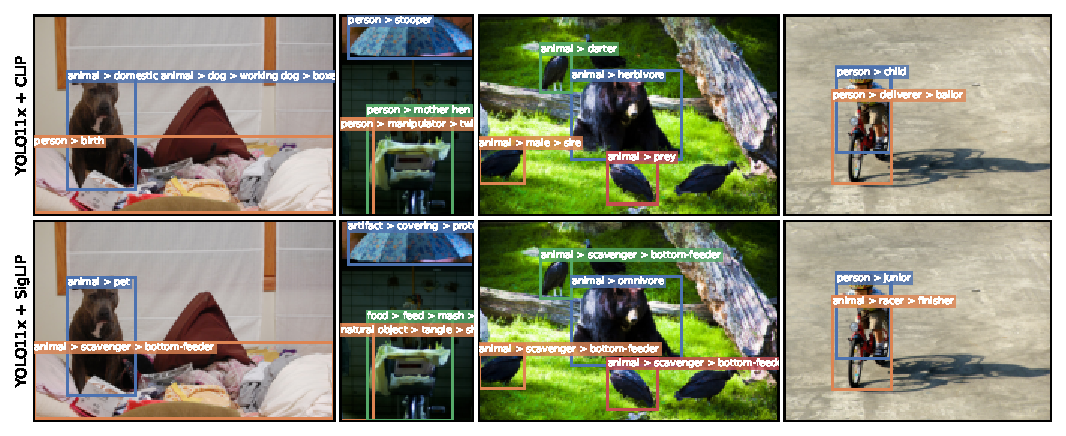
\includegraphics[width=0.8\linewidth]{figures/fig_qualitative.pdf}
    \caption{初期の語彙をWordNetの上位語6語とした定性評価の結果（上段：YOLO11x + CLIP，下段：YOLO11x + SigLIP，いずれも$ \theta = -1 $）．各ボックスに出力した単語の列を粗い語から順に示す．}
    \label{fig_qualitative}
\end{figure*}

図\ref{fig_qualitative}から，CLIPは犬をanimal → domestic animal → dog → working dog → boxerと，COCOのクラスであるdogを経由して犬種まで推定した．
SigLIPは傘をartifact → covering → protective covering → shade → parasolと推定した．
一方，同じ犬に対してSigLIPはanimal → petとし，熊にはanimal → omnivoreまたはherbivore，鳥にはanimal → scavenger → bottom-feederやanimal → preyが付けられた．
WordNetにおけるanimalの直接の下位語には，chordateのような分類学上の語に加えて，pet，herbivore，scavengerのように役割によって動物を分ける語が含まれ，これらの語にはさらに細かい下位語がほとんど無いため，細分化が浅い段階で止まった．
また，自転車にperson → deliverer → bailorやanimal → racer → finisherが付けられたように，最初の段階で物体と無関係な上位語を選ぶと，以降の単語も物体と無関係になった．

\subsection{COCO外の物体に対する評価の方法}
3.3節の提案手法を評価するため，COCOの画像に付与されたLVIS v1\cite{ref_LVIS}のアノテーションを用いた．
LVISは1203カテゴリのアノテーションを持ち，各カテゴリにWordNetのSynsetが付与されている．
LVISは，COCOで学習したYOLO11xをそのまま適用できるCOCOの画像に，COCOの80クラス以外の物体の正解とそのSynsetを与えるため，学習時に無い物体の命名を，上位語・下位語の関係を含めて自動で評価できる．
4.1節の検証用とテスト用の画像のうちLVISのアノテーションがある画像（検証用2387枚，テスト用2365枚）を用い，SynsetがCOCOのクラスのSynsetの上位語・下位語・自身のいずれでもなく，レンマもCOCOのクラス名と一致しない物体をCOCO外の物体（テスト用で13150件），それ以外をCOCOの物体（同11765件）とした．
出力したボックスとLVISのGTをIoU 0.5以上で1対1に対応付け，GTに出力が対応した割合を検出，出力した単語がGTのSynsetの上位語・自身・下位語のいずれかであった割合を命名，GTのSynset以下の単語まで細分化できた割合を細分化とした．
ただし，命名では深さ3未満の語とwholeを除いた．
また，出力した単語とGTのSynsetのそれぞれについて，自身と上位語のうち深さ3以上でwholeを除くSynsetの集合を求め，それらの重なりから階層的適合率$ hP $，階層的再現率$ hR $，およびその調和平均$ hF $を計算した\cite{ref_hF}．
GTと対応しない出力は全て誤りとし，このときの値を$ hP_{\mathrm{strict}} $，$ hF_{\mathrm{strict}} $とした．
ただし，LVISのアノテーションは全ての物体を網羅していないため，GTと対応しない出力には注釈の無い正しい物体も含まれる．
そこで上限の目安として，LVISの評価方法に倣い，画像に存在しないと確認されたカテゴリか，網羅的に注釈されたカテゴリの語またはその下位語を出力した場合のみ誤りとする$ hP_{\mathrm{fed}} $，$ hF_{\mathrm{fed}} $も求めた．
物体認識モデルにはYOLO11xを用い，3.3節の設定は検証用の画像で$ hF_{\mathrm{fed}} $が最大となるものを，$ \beta \in \{1, 2, 4, 8\} $，$ \tau \in \{0.05, 0.1, 0.2, \ldots, 0.9\} $，$ K \in \{10, 20, 50, 100\} $，$ o_{\min} \in \{0, 0.02, 0.05, 0.1, 0.2, 0.3\} $から，N1〜N4，A2の順に1段階ずつ選んだ．

OWLv2には，LVISの人手の注釈を学習に用いていないB/16の重み（自己学習のみ，以下ST）を主に用いた．
比較として，LVISの頻出カテゴリでファインチューニングした重み（以下FT）と，自己学習のみのL/14の重み（以下ST-L）も評価した．
FTは評価に用いるLVISのカテゴリの多くを学習時に見ているため，学習時に無い物体という本稿の目的に対しては参考値である．
なお，STもWeb上の画像と文章の大量の組による自己学習を行っているため，評価に用いる物体を一度も見ていないとは限らない．
本稿の「学習時に無い物体」は，LVISのカテゴリを正解のラベルとして学習していない物体を指す．

4.5節以降では，出力をスコアの順に並べた評価を行う．
スコアの高い順に出力をGTに対応付け（COCOのAPと同じ方法），スコアの閾値を下げながら出力を加えた場合の$ hR $と$ hP_{\mathrm{fed}} $，$ hP_{\mathrm{strict}} $から，適合率を単調にした曲線の面積をAP$ _{\mathrm{fed}} $，AP$ _{\mathrm{strict}} $とした．
階層的適合率・再現率は階層を持つ分類の評価に用いられる指標であり\cite{ref_hF}，粗い語の正しい出力に部分的な得点を与えるため，粒度を選ぶ手法の評価に適する．
本稿では，AP$ _{\mathrm{strict}} $を主な指標とし，AP$ _{\mathrm{fed}} $は上限の目安として示す．
一方，既存の物体認識の評価と比べるため，出力した単語がGTのSynset自身またはその下位語である出力のみを正解とするAP$ _{\mathrm{exact}} $も求めた．
AP$ _{\mathrm{exact}} $は，GTと対応しない出力を全て誤りとし，カテゴリを区別せずに全ての出力を1つの順位に並べたIoU 0.5のAPであり，LVISのカテゴリまで細分化した出力のみを正解とするため，通常のオープンボキャブラリの物体認識の評価に近い．
また，画像を単位として1000回の復元抽出を行うブートストラップ\cite{ref_Bootstrap}により，テスト用の画像における手法の間の差の95\%信頼区間を求めた．

\subsection{分類の能力と設定の影響}

\begin{table}[t]
    \vspace{3mm}
    \centering
    \caption{加えた領域のうちCOCO外の物体と重なるものについて，OWLv2の1位の単語が正しかった割合（テスト用）．括弧内は正しい上位語・下位語を含む割合である．LVISの語彙は正解の語を必ず含む．}
    \label{tab_diag}
    \footnotesize
    \begin{tabular}{lccc}
        \toprule
        OWLv2 & 領域数 & LVIS（1202語） & キャプション（7806語） \\
        \midrule
        ST & 1869 & 0.411 (0.468) & 0.180 (0.241) \\
        ST-L & 1450 & 0.438 (0.496) & 0.170 (0.218) \\
        FT & 3812 & 0.705 (0.762) & 0.477 (0.560) \\
        \bottomrule
    \end{tabular}
\end{table}

表\ref{tab_diag}に，加えた領域（$ K = 10 $）のうちCOCO外の物体と重なるものに対する，OWLv2の分類の正解率を示す．
FTはLVISの語彙で70.5\%であったのに対し，STは41.1\%，ST-Lは43.8\%であり，以前の版で観測した高い分類能力の多くはLVISによるファインチューニングに由来していた．
また，正解を含む1202語から7806語に語彙を広げると，正解率はSTで18.0\%に下がった．
したがって，学習時に無い物体を扱う条件では，語彙全体からの1語の選択は信頼できず，確信度に応じて粗い語で止める必要がある．

\begin{table}[t]
    \vspace{3mm}
    \centering
    \caption{STを用いた場合のテスト用の画像における評価．各行は1つ上の行の設定に変更を加えたものである．$ hF_{\mathrm{fed}} $は設定の選択に用いた指標である．}
    \label{tab_open}
    \footnotesize
    \setlength{\tabcolsep}{2pt}
    \begin{tabular}{lcccc}
        \toprule
        & \multicolumn{3}{c}{COCO外の物体} & \\
        \cmidrule(lr){2-4}
        構成 & 検出 & 命名 & 細分化 & $ hF_{\mathrm{fed}} $ \\
        \midrule
        flat & 0.212 & 0.034 & {\bf 0.033} & 0.377 \\
        deepest & 0.212 & 0.057 & 0.022 & 0.380 \\
        backoff & 0.212 & {\bf 0.063} & 0.013 & 0.386 \\
        greedy (N3) & 0.212 & 0.053 & 0.014 & 0.391 \\
        + N4 & 0.212 & 0.055 & 0.019 & 0.395 \\
        \midrule
        + $ K{=}20 $ & 0.302 & 0.094 & 0.034 & 0.423 \\
        + $ K{=}50 $ & 0.454 & 0.164 & 0.056 & 0.466 \\
        + $ K{=}100 $$ ^\dagger $ & {\bf 0.560} & {\bf 0.211} & {\bf 0.073} & {\bf 0.494} \\
        \bottomrule
    \end{tabular}
\end{table}

表\ref{tab_open}に，STを用いた場合の各段階の結果を示す（$ K = 10 $から開始し，$ ^\dagger $は$ o_{\min} = 0.02 $）．
確率が最大の単語をそのまま出力するflatは細分化が最も高いが命名は3.4\%であり，誤った細かい語が多かった．
上位語への集約（N2）と組み合わせると命名は5.3〜6.3\%に上がり，検証用の画像ではgreedy（$ \beta = 2 $，$ \tau = 0.1 $）が選ばれた．
語義を区別する文章と人の役割の除外（N4）により，細分化は1.4\%から1.9\%に向上した．
YOLO11xのボックスをクラスの下位語へ細分化する設定も評価したが，検証用の画像では細分化しない設定が選ばれた．
最も効果が大きかったのは加える領域の数$ K $であり，$ K = 100 $でCOCO外の物体の検出は21.2\%から56.0\%に，命名は5.5\%から21.1\%に，細分化は1.9\%から7.3\%に向上した．
一方で，加えた領域の多くは物体でない領域であった（4.7節）．

$ K $と$ o_{\min} $を$ hF_{\mathrm{strict}} $で選ぶと$ o_{\min} = 0.3 $となり，加える領域は1画像あたり2.0件に減り，COCO外の物体の命名は1.8\%にとどまった．
同じ設定（$ K = 100 $）で，ST-Lでは細分化が13.3\%とSTより高く，命名はSTと同程度の20.3\%であった．
FTでは命名35.5\%，細分化28.1\%となり，STとの差はLVISによるファインチューニングの効果を含む．
このように，$ K $と$ o_{\min} $のみでは命名を保ちながら誤った出力を減らすことは難しく，4.6節ではスコアによって出力を選ぶ．

\subsection{命名の方法の比較}
上位語への集約と確信度に応じた停止の効果を，階層を用いずに確率が最大の1語を出力する方法（flat）と比較した．
さらに，評価の語彙を事前に知る場合の参考として，OWLv2にLVISの1203カテゴリ名を語彙として与え，同じ2つの規則で命名した場合も評価した．
これは，評価するクラスの集合を与えるという，オープンボキャブラリの物体認識モデルの通常の使い方に相当する．
いずれもYOLO11xのボックスの出力は同じであり，加えた領域（$ K = 100 $）の命名のみが異なる．
各方法には，3.3節の(\ref{eq_score})のスコアを方法ごとに検証用の画像で重みを求めて付け，スコアの順の曲線で比較した．

\begin{table}[t]
    \vspace{3mm}
    \centering
    \caption{命名の方法ごとのテスト用の画像における評価．スコアは(\ref{eq_score})である．LVISの語彙は評価のカテゴリ名を事前に与える場合（参考）である．AP$ _{\mathrm{fed}} $は上限の目安である．}
    \label{tab_baseline}
    \footnotesize
    \setlength{\tabcolsep}{3pt}
    \begin{tabular}{lllccc}
        \toprule
        OWLv2 & 語彙 & 規則 & AP$ _{\mathrm{strict}} $ & AP$ _{\mathrm{exact}} $ & AP$ _{\mathrm{fed}} $ \\
        \midrule
        ST & キャプション & flat & 0.193 & {\bf 0.104} & 0.306 \\
         & キャプション & greedy & {\bf 0.197} & 0.096 & {\bf 0.333} \\
         & LVIS & flat & 0.209 & 0.116 & 0.351 \\
         & LVIS & greedy & 0.208 & 0.111 & 0.354 \\
        \midrule
        ST-L & キャプション & flat & 0.188 & {\bf 0.104} & 0.310 \\
         & キャプション & greedy & {\bf 0.191} & 0.102 & {\bf 0.331} \\
         & LVIS & flat & 0.203 & 0.119 & 0.362 \\
         & LVIS & greedy & 0.205 & 0.118 & 0.367 \\
        \midrule
        FT & キャプション & flat & 0.264 & 0.160 & 0.430 \\
         & キャプション & greedy & {\bf 0.277} & {\bf 0.161} & {\bf 0.456} \\
         & LVIS & flat & 0.316 & 0.220 & 0.511 \\
         & LVIS & greedy & 0.313 & 0.215 & 0.508 \\
        \bottomrule
    \end{tabular}
\end{table}

表\ref{tab_baseline}に結果を示す．
キャプションの語彙では，greedyはflatに比べ，全ての重みでAP$ _{\mathrm{strict}} $が0.003〜0.013高かった．
ブートストラップによる差の95\%信頼区間は，STで0.001〜0.009，FTで0.008〜0.019であり，いずれも0を含まなかったが，差は小さい．
一方，LVISのカテゴリまで正しい出力のみを数えるAP$ _{\mathrm{exact}} $は，STでflatの方が0.008（95\%信頼区間0.007〜0.010）高く，FTでは差が無かった（$-0.003$〜0.005）．
これは，greedyが確信度の低い領域で粗い語に止まり，細かい語での正解を一部失うためである．

この違いを領域ごとに確かめるため，テスト用の画像で検出のスコアの順にCOCO外の物体と対応した加えた領域（STで6385件）について，同じ領域に対する2つの方法の命名の正誤を比べた．
命名が正しかった割合は，flatの25.9\%に対しgreedyで43.0\%であった．
greedyのみが正しかった領域は1551件，flatのみが正しかった領域は457件であり，前者には，jerseyに対するflatのjerseyとgreedyのshirt，skirtに対するshort pantsとgarment，ringに対するbandとjewelryのように，flatが誤った細かい語を選び，greedyが正しい上位語に止まった例が多かった．
後者には，handleに対するknobとfastenerのように，greedyが最初の段階で誤った枝に進んだ例が多かった．
ST-Lでは42.2\%と29.7\%，FTでは56.2\%と48.9\%であり，分類の能力が高い重みほど差は小さかった．
すなわち，上位語への集約は領域ごとの命名の正しさを大きく改善するが，その多くは粗い語による正解であり，出力全体のAPへの寄与は小さい．

また，評価の語彙を事前に与えると，AP$ _{\mathrm{strict}} $はSTで0.193〜0.197から0.208〜0.209に，FTで0.264〜0.277から0.313〜0.316に向上した．
語彙が1203語に限られ正解の語を必ず含む場合には，greedyとflatの差は小さく，FTではflatが有意に高かった（AP$ _{\mathrm{strict}} $で0.003，95\%信頼区間0.001〜0.004）．
したがって，上位語への集約が有効なのは，評価の語彙を事前に知らず，大きな語彙から命名する場合である．

\subsection{アノテーションのスコアの評価}
3.3節のスコアの効果を評価するため，4.4節で選んだ設定（$ K = 100 $，$ o_{\min} = 0 $）の全ての出力にスコアを付け，4.3節のAP$ _{\mathrm{strict}} $とAP$ _{\mathrm{fed}} $を求めた．
また，スコアを確率とみなし，正誤が判定できる出力（GTと対応した出力と，$ hF_{\mathrm{fed}} $で誤りとした出力）について，10個のビンで期待校正誤差（Expected Calibration Error，ECE）\cite{ref_Calibration}を求めた．
比較として，学習を伴わない検出のスコア$ c({\mathbf b}) $，命名の確率$ q(n \mid {\mathbf b}) $，両者の積，および加えた領域のみ両者の積とする場合を評価した．
(\ref{eq_score})の重みは検証用の画像の18488件の出力（正の割合45.7\%）で求めた．

\begin{table}[t]
    \vspace{3mm}
    \centering
    \caption{スコアの種類ごとのテスト用の画像における評価．$ ^\dagger $は加えた領域のみ積とし，YOLO11xのボックスは$ c $とした場合である．AP$ _{\mathrm{fed}} $は上限の目安である．}
    \label{tab_score}
    \footnotesize
    \setlength{\tabcolsep}{4pt}
    \begin{tabular}{llccc}
        \toprule
        OWLv2 & スコア & AP$ _{\mathrm{strict}} $ & ECE & AP$ _{\mathrm{fed}} $ \\
        \midrule
        ST & $ c $ & 0.171 & 0.145 & 0.323 \\
        ST & $ q $ & 0.042 & 0.339 & 0.272 \\
        ST & $ c \cdot q $ & 0.116 & 0.436 & 0.301 \\
        ST & $ c \cdot q^\dagger $ & 0.171 & 0.231 & 0.324 \\
        ST & $ s $ & {\bf 0.197} & {\bf 0.028} & {\bf 0.333} \\
        \midrule
        ST-L & $ c $ & 0.162 & 0.146 & 0.320 \\
        ST-L & $ s $ & 0.191 & 0.025 & 0.331 \\
        FT & $ c $ & 0.243 & 0.168 & 0.438 \\
        FT & $ s $ & 0.277 & 0.013 & 0.456 \\
        \bottomrule
    \end{tabular}
\end{table}

\begin{figure*}[t]
    \centering
    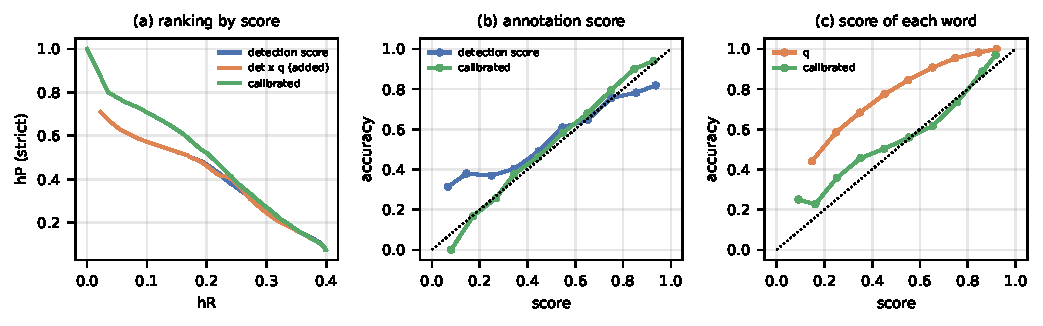
\includegraphics[width=0.8\textwidth]{figures/fig_score.pdf}
    \caption{STを用いた場合のテスト用の画像におけるスコアの評価．(a)スコアの順に出力を加えた場合の$ hR $と$ hP_{\mathrm{strict}} $，(b)アノテーションのスコアの値（横軸）と正解率（縦軸）の関係，(c)GTと対応した加えた領域の経路上の各単語の集約した確率$ q $と(\ref{eq_word_score})のスコアの値と正解率の関係．点線は完全に校正された場合である．}
    \label{fig_score}
\end{figure*}

表\ref{tab_score}と図\ref{fig_score}に結果を示す．
命名の確率$ q $のみでは，物体でない領域にも高い値が付くためAP$ _{\mathrm{strict}} $は0.042と低く，検出のスコアとの積でもYOLO11xのボックスの$ q $が低いため検出のスコアのみより低下した．
加えた領域のみ積とすると，学習を伴わずに検出のスコアと同程度以上となった．
(\ref{eq_score})のスコア$ s $は，全ての重みでAP$ _{\mathrm{strict}} $とAP$ _{\mathrm{fed}} $が最も高く，STではAP$ _{\mathrm{strict}} $が0.171から0.197に向上した．
また，ECEは0.145から0.028に低下し，図\ref{fig_score}(b)のようにスコアの値が正解率とほぼ一致した．
経路上の各単語では，集約した確率$ q $は正解率より低く（ECE 0.275），(\ref{eq_word_score})のスコアによりECEは0.041に低下した（ST-Lで0.172から0.062，FTで0.244から0.041）．
この改善は偶然によるものではなく，ブートストラップによるSTのAP$ _{\mathrm{strict}} $の差は0.026（95\%信頼区間0.021〜0.031），FTでは0.034（0.028〜0.041）であった．

\begin{figure*}[t]
    \centering
    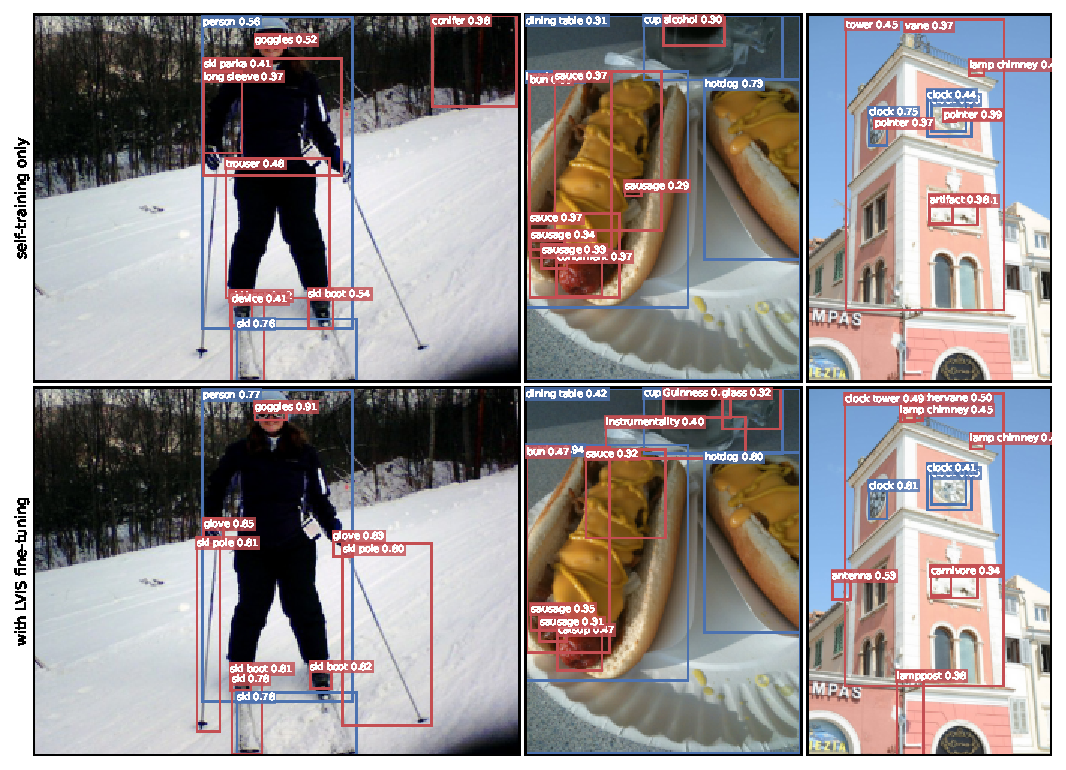
\includegraphics[width=0.62\textwidth]{figures/fig_qualitative_open.pdf}
    \caption{テスト用の画像における出力の例（上段：ST，下段：FT）．青はYOLO11xのボックスとクラス，赤は加えた領域のうち(\ref{eq_score})のスコアが高い上位8件と，3.3節の方法で選んだ単語，数値はそのスコアである．}
    \label{fig_qualitative_open}
\end{figure*}

図\ref{fig_qualitative_open}に出力の例を示す．
STでも，スキーの画像のgoggles（0.52），ski boot（0.54），trouser（0.48），ski parka（0.41），ホットドッグの画像のsausage，sauce，時計塔の画像のtower（0.45）のように，COCO外の物体に正しい単語とスコアが付けられた．
例えばski parkaの領域の経路上の各単語のスコアは，artifact 0.89，clothing 0.89，jacket 0.82，parka 0.62，ski parka 0.43であり，粗い語ほど高い．
一方，STではalcohol（0.30）のような誤りも残り，FTではgoggles（0.91），glove（0.85），ski pole（0.81）のように正しい細かい語に高いスコアが付けられた．

\subsection{誤りの分解}
提案手法の精度を制限する要因を調べるため，テスト用の画像における加えた領域の出力を，スコアの順にGTへ対応付けた結果から6種類に分けた．
GTと対応し命名が正しい出力を正しい命名，GTと対応したが命名が誤りの出力を誤った命名，IoUが0.5以上のGTが既に他の出力に対応していた出力を重複とした．
GTと対応しない残りの出力は，領域の面積の80\%以上がいずれかのGTのボックスに含まれる場合を物体の一部，GTとの最大のIoUが0.1以上0.5未満の場合を位置ずれ，それ以外を背景とした．
ただし，LVISのアノテーションは網羅的でないため，物体の一部と背景には注釈の無い物体も含まれる．

\begin{table}[t]
    \vspace{3mm}
    \centering
    \caption{加えた領域の出力の種類の割合（\%，テスト用）．「全て」は$ K = 100 $の全ての出力，「閾値」は検証用の画像で$ hF_{\mathrm{strict}} $が最大となる(\ref{eq_score})の閾値以上の出力である．}
    \label{tab_errors}
    \footnotesize
    \setlength{\tabcolsep}{1.5pt}
    \begin{tabular}{lccccccc}
        \toprule
        構成 & 出力数 & 正しい & 誤り & 重複 & 一部 & 位置 & 背景 \\
        \midrule
        ST greedy 全て & 220899 & 1.8 & 2.3 & 0.5 & 35.0 & 9.8 & 50.8 \\
        ST greedy 閾値 & 4657 & 16.6 & 5.8 & 0.9 & 31.1 & 13.0 & 32.6 \\
        ST flat 閾値 & 3763 & 17.3 & 11.0 & 0.7 & 28.2 & 14.8 & 27.9 \\
        FT greedy 閾値 & 14489 & 26.6 & 10.0 & 0.4 & 23.2 & 8.4 & 31.5 \\
        \bottomrule
    \end{tabular}
\end{table}

表\ref{tab_errors}に結果を示す．
STで$ K = 100 $の全ての出力のうち，GTと対応した出力は4.1\%にすぎず，物体の一部が35.0\%，背景が50.8\%を占めた．
閾値以上の出力に限っても，物体の一部，位置ずれ，背景の合計は76.7\%であり，誤った命名は5.8\%であった．
flatでは誤った命名が11.0\%とgreedyの約2倍であり，greedyは命名の誤りを粗い語に止まることで減らしていた．
すなわち，提案手法の誤りの多くは，命名ではなく，物体の全体でない領域を加えることに起因する．

この要因の大きさを見積もるため，GTを用いて，いずれかのGTとIoUが0.5以上で重なる加えた領域のみを残した場合を評価した．
これはGTを用いるため手法ではなく，領域の追加が完全な場合の上限である．
STで(\ref{eq_score})のスコアを用いると，AP$ _{\mathrm{strict}} $はgreedyで0.197から0.265に，flatで0.193から0.237に向上した．
物体でない領域が除かれると，greedyとflatの差はAP$ _{\mathrm{strict}} $で0.004から0.028に広がった．
ST-Lでは0.264と0.239，FTでは0.401と0.365であり，FTではAP$ _{\mathrm{exact}} $もgreedyが0.228とflatの0.222を上回った．
したがって，物体でない領域を区別する方法が得られれば，上位語への集約による命名の改善が出力全体の精度により大きく反映される．

\begingroup
\color{red}
\begin{table}[t]
    \vspace{3mm}
    \centering
    \caption{\add{全体らしさの特徴を(\ref{eq_score})に加えた場合のAP$ _{\mathrm{strict}} $（テスト用，greedy）．括弧内は加えない場合との差の95\%信頼区間である．}}
    \label{tab_whole}
    \color{red}
    \footnotesize
    \setlength{\tabcolsep}{2pt}
    \begin{tabular}{lcccc}
        \toprule
        特徴 & \multicolumn{2}{c}{ST} & \multicolumn{2}{c}{FT} \\
        \midrule
        加えない & 0.197 & --- & 0.277 & --- \\
        ＋幾何 & 0.200 & [$+$0.002, $+$0.004] & 0.280 & [$+$0.001, $+$0.004] \\
        ＋WordNet & 0.196 & [$-$0.003, 0.000] & 0.274 & [$-$0.005, $-$0.001] \\
        ＋両方 & 0.199 & [0.000, $+$0.003] & 0.276 & [$-$0.003, 0.000] \\
        規則で棄却 & 0.197 & [0.000, $+$0.001] & 0.277 & [$-$0.002, $+$0.001] \\
        \bottomrule
    \end{tabular}
\end{table}

そこで，GTを用いずに物体の全体でない領域を区別することを試みた．
加えた領域ごとに，面積が1.5倍以上のYOLO11xのボックスおよび全てのボックスに含まれる割合の最大値，内側に含む加えた領域の数，画像内で最大のボックスに対する面積の比の4個を幾何の特徴とした．
また，面積の80\%以上を含む大きなボックスの経路上の語の部分（WordNetのpart meronymを推移的にたどったもの）に出力した語が当たるか，および出力した語が何かの部分を表す語かの2個をWordNetの特徴とした．
例えば，carのボックスに含まれるwheelの領域は前者が真となる．
これらを(\ref{eq_score})の特徴に加えて検証用の画像で重みを求め直した場合と，前者が真の領域を棄却する規則のみの場合の結果を表\ref{tab_whole}に示す．
幾何の特徴によりAP$ _{\mathrm{strict}} $はSTとFTで約0.002向上したが，ST-Lでは0.191から0.189に低下し，WordNetの特徴はいずれの場合も精度を向上させなかった．
part meronymが真となった領域のうち正しい出力は1〜2\%にすぎなかったが，物体の一部の出力のうち該当するものは9〜11\%であり，規則による棄却でも閾値以上の出力に占める物体の一部の割合は31.1\%から28.5\%に減るのみであった．
また，正しい出力の領域もYOLO11xのボックスに含まれる割合が平均0.63と高く（物体の一部は0.86），人の衣服のように大きな物体に含まれる物体と，物体の一部とを位置関係と語の関係のみでは区別できなかった．
\endgroup

\section{考察}
\subsection{予備実験から分かること}
予備実験では，同じボックスを用いて物体認識モデル自身のクラスと文章・画像埋め込みモデルによるクラスを比較したため，両者の差は全てクラスの推定に起因する．
COCOの80クラスの範囲では，COCOで学習した物体認識モデルのラベルの一致率は0.95以上であり，ゼロショット分類の0.56〜0.58を大きく上回った．
したがって，学習時のクラスの範囲では物体認識モデル自身のクラスを用いるべきであり，文章・画像埋め込みモデルの利点は，学習時に無い物体と語彙を追加の学習なしに扱える点にある．
また，WordNetの上位語から1段ずつ下位語を選ぶ方法では，役割を表す下位語に進んで細分化が止まる誤りと，最初の段階の誤りが以降の全ての段階に伝播する誤りが見られた．
提案手法は，前者を人の役割の語の除外と語義を区別する文章で，後者を語彙全体の確率の上位語への集約で緩和するものである．

\subsection{上位語への集約の効果と限界}
4.5節から，上位語への集約による命名は，同じ領域に対する命名の正しさを25.9\%から43.0\%に改善した．
これは，表\ref{tab_diag}のように学習時に無い物体に対する1位の単語の正解率が低くても，正解の語とその近くの語の確率が共通の上位語に集まるためである．
一方，改善の多くは粗い語による正解であり，LVISのカテゴリまで正しい出力のみを数えるAP$ _{\mathrm{exact}} $ではflatが上回った．
すなわち，提案手法は細かい語の正解を増やす方法ではなく，誤った細かい語を正しい粗い語に置き換える方法であり，その効果は階層的な指標でのみ現れる．
また，評価の語彙を事前に与えた場合には集約の効果は無かった．
語彙が小さく正解の語を必ず含む場合には，1位の単語の正解率が高く，粗い語に止まる利点が小さいためと考えられる．
したがって，提案手法が有効なのは，評価の語彙を事前に知らず，学習時に無い物体を大きな語彙から命名する場合である．
細かい語の正解を増やすには，ST-LやFTとの比較から分かるように，領域の特徴の分類能力そのものを高める必要がある．

\subsection{実用上の水準と誤りの要因}
提案手法の出力は，そのままでは人手のアノテーションの代わりにはならない．
STを用いて検証用の画像で選んだ閾値を用いると，閾値以上の加えた領域の出力のうち正しく命名されたものは16.6\%（表\ref{tab_errors}）であり，COCO外の物体のうち命名できたものは3.2\%であった．
一方，(\ref{eq_score})のスコアはテスト用の画像で正解率とほぼ一致したため，スコアが高い出力のみを候補として人に示し，確認させる用途には利用できる．
4.7節の誤りの分解から，加えた領域の出力の誤りの大部分は命名ではなく物体の一部や背景に対するものであり，GTと重なる領域のみを残すとAP$ _{\mathrm{strict}} $は0.197から0.265に向上した．
したがって，次に改善すべきは命名ではなく，領域が物体の全体であるかの判定である．
なお，LVISのアノテーションは網羅的でないため，GTと対応しない出力の全てが誤りとは限らず，$ hF_{\mathrm{fed}} $と$ hF_{\mathrm{strict}} $，およびAP$ _{\mathrm{fed}} $とAP$ _{\mathrm{strict}} $は真の値の上限と下限に近いと考えられる．
また，スコアの重みはLVISの検証用の画像で求めたため，LVISと異なる分布の画像では校正が崩れる可能性がある．

\subsection{今後の課題}
第一に，領域が物体の全体であるかを判定し，物体の一部や背景の領域を棄却することが挙げられる．
\add{4.7節のように，ボックスの包含関係や大きさ，WordNetの部分と全体の関係のみでは効果が小さかったため，領域の周囲を含めて切り抜いた画像の特徴の変化等，画像の内容に基づく判定が必要である．}
第二に，学習時に無い物体に対する領域の特徴の分類能力の向上が挙げられ，より規模の大きい文章・画像埋め込みモデルの特徴と組み合わせる方法が考えられる．
第三に，LVISのアノテーションの網羅性の不足を補うため，GTと対応しない出力を人手で確認し，真の適合率を求めることが挙げられる．

\section{おわりに}
本稿では，モデルの再学習を行わずに，学習時に無い物体を検出し，確信度に応じた粒度で命名する粒度可変アノテーションを提案した．
提案手法は，YOLO11xのボックスにOWLv2の領域を加え，領域の特徴から求めた7806語の確率をWordNetの上位語へ集約して上位語から貪欲に下位語へ進み，各アノテーションと経路上の各単語に正しさの確率を付ける．
LVISの人手の注釈を学習に用いていないOWLv2による評価では，COCO外の物体の検出は56.0\%，命名は21.1\%であった．
同じ領域に対する命名の正しさは，確率が最大の1語を出力する場合の25.9\%から43.0\%に向上し，提案したスコアは期待校正誤差を0.145から0.028に下げ，全ての誤りを数えるAPを0.171から0.197に高めた．
これらの差は，ブートストラップによる信頼区間で確認した．
一方，改善の多くは粗い語による正解であり，LVISのカテゴリまで正しい出力のみを数える評価や，評価の語彙を事前に与えた場合には，集約の効果は無かった．
また，誤りの大部分は物体の一部や背景の領域に対するものであり，\add{ボックスの位置関係とWordNetの部分と全体の関係を用いてこれらを棄却する方法では，APの向上は0.003以下に止まった．}
今後は，領域が物体の全体であるかの判定，領域の特徴の分類能力の向上，およびGTと対応しない出力の人手による確認に取り組む．

\vspace{-1mm}
\begin{thebibliography}{99}

    \bibitem{ref_YOLO}
    J. Redmon, S. Divvala, R. Girshick, and A. Farhadi,
    ``You Only Look Once: Unified, Real-Time Object Detection,''
    in {\it Proc. IEEE Conference on Computer Vision and Pattern Recognition (CVPR)}, 2016.

    \bibitem{ref_DETR}
    N. Carion, F. Massa, G. Synnaeve, N. Usunier, A. Kirillov, and S. Zagoruyko,
    ``End-to-End Object Detection with Transformers,''
    in {\it Proc. European Conference on Computer Vision (ECCV)}, 2020.

    \bibitem{ref_CLIP}
    A. Radford, J. W. Kim, C. Hallacy, A. Ramesh, G. Goh, S. Agarwal, G. Sastry, A. Askell, P. Mishkin, J. Clark, G. Krueger, and I. Sutskever,
    ``Learning Transferable Visual Models From Natural Language Supervision,''
    in {\it Proc. International Conference on Machine Learning (ICML)}, 2021.

    \bibitem{ref_SigLIP}
    X. Zhai, B. Mustafa, A. Kolesnikov, and L. Beyer,
    ``Sigmoid Loss for Language Image Pre-Training,''
    in {\it Proc. IEEE/CVF International Conference on Computer Vision (ICCV)}, pp. 11975--11986, 2023.

    \bibitem{ref_WordNet}
    G. A. Miller,
    ``WordNet: A Lexical Database for English,''
    {\it Communications of the ACM}, vol. 38, no. 11, pp. 39--41, 1995.

    \bibitem{ref_COCO}
    T.-Y. Lin, M. Maire, S. Belongie, J. Hays, P. Perona, D. Ramanan, P. Doll\'{a}r, and C. L. Zitnick,
    ``Microsoft COCO: Common Objects in Context,''
    in {\it Proc. European Conference on Computer Vision (ECCV)}, 2014.

    \bibitem{ref_YOLO11}
    G. Jocher, J. Qiu, and A. Chaurasia,
    ``Ultralytics YOLO,''
    2023, \url{https://github.com/ultralytics/ultralytics}.

    \bibitem{ref_OWLViT}
    M. Minderer, A. Gritsenko, A. Stone, M. Neumann, D. Weissenborn, A. Dosovitskiy, A. Mahendran, A. Arnab, M. Dehghani, Z. Shen, X. Wang, X. Zhai, T. Kipf, and N. Houlsby,
    ``Simple Open-Vocabulary Object Detection with Vision Transformers,''
    in {\it Proc. European Conference on Computer Vision (ECCV)}, 2022.

    \bibitem{ref_GroundingDINO}
    S. Liu, Z. Zeng, T. Ren, F. Li, H. Zhang, J. Yang, C. Li, J. Yang, H. Su, J. Zhu, and L. Zhang,
    ``Grounding DINO: Marrying DINO with Grounded Pre-Training for Open-Set Object Detection,''
    in {\it Proc. European Conference on Computer Vision (ECCV)}, 2024.

    \bibitem{ref_OpenCLIP}
    G. Ilharco, M. Wortsman, R. Wightman, C. Gordon, N. Carlini, R. Taori, A. Dave, V. Shankar, H. Namkoong, J. Miller, H. Hajishirzi, A. Farhadi, and L. Schmidt,
    ``OpenCLIP,''
    2021, \url{https://github.com/mlfoundations/open_clip}.

    \bibitem{ref_Hungarian}
    H. W. Kuhn,
    ``The Hungarian Method for the Assignment Problem,''
    {\it Naval Research Logistics Quarterly}, vol. 2, no. 1--2, pp. 83--97, 1955.

    \bibitem{ref_OWLv2}
    M. Minderer, A. Gritsenko, and N. Houlsby,
    ``Scaling Open-Vocabulary Object Detection,''
    in {\it Proc. Advances in Neural Information Processing Systems (NeurIPS)}, 2023.

    \bibitem{ref_LVIS}
    A. Gupta, P. Doll\'{a}r, and R. Girshick,
    ``LVIS: A Dataset for Large Vocabulary Instance Segmentation,''
    in {\it Proc. IEEE/CVF Conference on Computer Vision and Pattern Recognition (CVPR)}, pp. 5356--5364, 2019.

    \bibitem{ref_hF}
    S. Kiritchenko, S. Matwin, R. Nock, and A. F. Famili,
    ``Learning and Evaluation in the Presence of Class Hierarchies: Application to Text Categorization,''
    in {\it Proc. Canadian Conference on Artificial Intelligence}, pp. 395--406, 2006.

    \bibitem{ref_Hedging}
    J. Deng, J. Krause, A. C. Berg, and L. Fei-Fei,
    ``Hedging Your Bets: Optimizing Accuracy-Specificity Trade-offs in Large Scale Visual Recognition,''
    in {\it Proc. IEEE Conference on Computer Vision and Pattern Recognition (CVPR)}, pp. 3450--3457, 2012.

    \bibitem{ref_CHiLS}
    Z. Novack, J. McAuley, Z. C. Lipton, and S. Garg,
    ``CHiLS: Zero-Shot Image Classification with Hierarchical Label Sets,''
    in {\it Proc. International Conference on Machine Learning (ICML)}, pp. 26342--26362, 2023.

    \bibitem{ref_Platt}
    J. Platt,
    ``Probabilistic Outputs for Support Vector Machines and Comparisons to Regularized Likelihood Methods,''
    in {\it Advances in Large Margin Classifiers}, MIT Press, pp. 61--74, 1999.

    \bibitem{ref_Calibration}
    C. Guo, G. Pleiss, Y. Sun, and K. Q. Weinberger,
    ``On Calibration of Modern Neural Networks,''
    in {\it Proc. International Conference on Machine Learning (ICML)}, pp. 1321--1330, 2017.

    \bibitem{ref_Bootstrap}
    B. Efron and R. J. Tibshirani,
    {\it An Introduction to the Bootstrap}, Chapman \& Hall, 1993.

\end{thebibliography}


\end{document}
